\documentclass[10pt,a4paper]{article}
\usepackage[T1]{fontenc}
\usepackage{lmodern,microtype}
\usepackage[margin=22mm,headheight=14pt]{geometry}
\usepackage{amsmath,amssymb,mathtools,booktabs,tabularx,longtable}
\usepackage[dvipsnames]{xcolor}
\usepackage{tikz}
\usetikzlibrary{arrows.meta,positioning,shapes.geometric}
\usepackage{fancyhdr}
\usepackage[colorlinks=true,linkcolor=MidnightBlue,citecolor=MidnightBlue,urlcolor=MidnightBlue]{hyperref}
\hypersetup{pdftitle={APi-TOF simulation: model and numerical methods},pdfauthor={apitofsim contributors}}
\pagestyle{fancy}
\fancyhf{}
\fancyhead[L]{\small APi-TOF simulation}
\fancyhead[R]{\small Model and numerical methods}
\fancyfoot[C]{\thepage}
\setlength{\parindent}{0pt}
\setlength{\parskip}{5pt plus 1pt}
\setlength{\emergencystretch}{1em}
\newcommand{\dd}{\,\mathrm d}
\newcommand{\kb}{k_{\mathrm B}}
\newcommand{\Normal}{\mathcal N}
\newcommand{\Unif}{\operatorname{Unif}}
\newcommand{\Exp}{\operatorname{Exp}}
\newcommand{\Dir}{\operatorname{Dirichlet}}
\newcommand{\erf}{\operatorname{erf}}
\newcommand{\code}[1]{\href{https://github.com/VilmaLab/apitofsim/blob/main/#1}{\nolinkurl{#1}}}
\newcommand{\overview}[2]{\section*{#1\quad #2}\addcontentsline{toc}{section}{#1 #2}}
\newenvironment{steps}{\begin{enumerate}\setlength{\itemsep}{3pt}\setlength{\parskip}{0pt}}{\end{enumerate}}
\tikzset{box/.style={draw=MidnightBlue,rounded corners,fill=blue!4,align=center,inner sep=7pt},arr/.style={-{Stealth},thick,draw=MidnightBlue}}

\begin{document}
\begin{center}
{\LARGE\bfseries APi-TOF simulation}\par\vspace{4pt}
{\large Model and numerical methods}\par\vspace{3pt}
{\small A mathematical description of preprocessing, event dynamics and serial fragmentation}
\end{center}

\overview{1}{The pipeline}
An atmospheric pressure interface time-of-flight (APi-TOF) mass spectrometer
accelerates charged molecular clusters through residual carrier gas. Gas collisions
transfer translational energy into internal excitation, enabling fragmentation.
The model follows independent ion realizations through the simulated interface,
not through the full flight tube or detector electronics. Its foundations are
kinetic gas theory, microcanonical energy partition and phase-space detailed
balance~\cite{zapadinsky,si,zanca}; experimental applications include
Ref.~\cite{alfaouri}.

\begin{center}
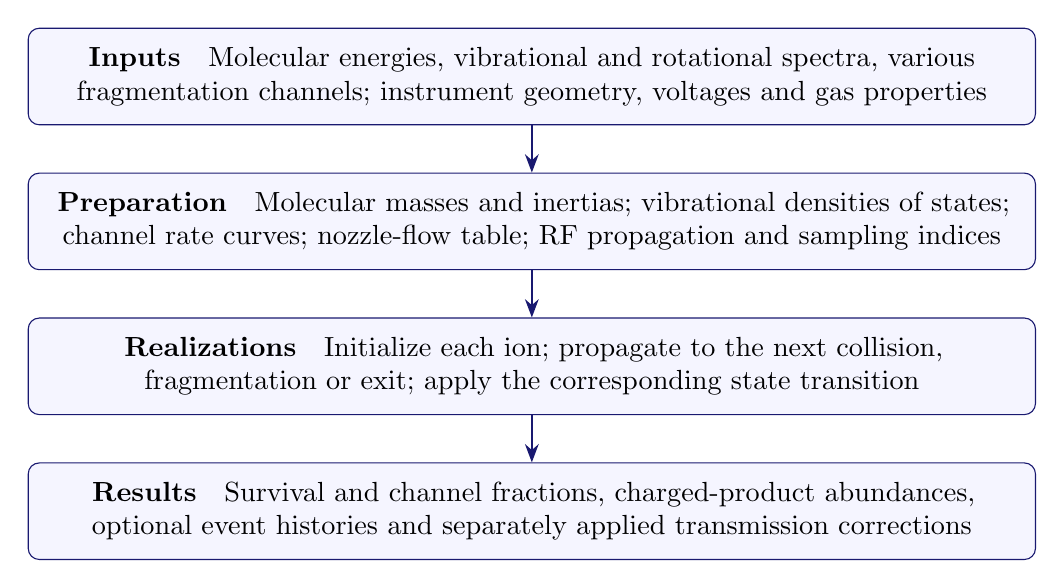
\begin{tikzpicture}[node distance=6mm]
\node[box,text width=12.3cm] (in) {\textbf{Inputs}\quad Molecular energies, vibrational and rotational spectra,\ various fragmentation channels; instrument geometry, voltages and gas properties};
\node[box,text width=12.3cm,below=of in] (prep) {\textbf{Preparation}\quad Molecular masses and inertias; vibrational densities of states;\ channel rate curves; nozzle-flow table; RF propagation and sampling indices};
\node[box,text width=12.3cm,below=of prep] (run) {\textbf{Realizations}\quad Initialize each ion; propagate to the next collision,\ fragmentation or exit; apply the corresponding state transition};
\node[box,text width=12.3cm,below=of run] (out) {\textbf{Results}\quad Survival and channel fractions, charged-product abundances,\ optional event histories and separately applied transmission corrections};
\draw[arr] (in)--(prep); \draw[arr] (prep)--(run); \draw[arr] (run)--(out);
\end{tikzpicture}
\end{center}

The dynamical state is
\[
 X=(i,\mathbf r,\mathbf v,\boldsymbol\omega,E_v,t),\qquad
 E_r=\tfrac12 I_i|\boldsymbol\omega|^2,\qquad E=E_v+E_r.
\]
Here $i$ identifies the current cluster, $\mathbf r=(x,y,z)$ is position,
$\mathbf v$ its velocity, $\boldsymbol\omega$ its angular velocity, $I_i$ its
spherical moment of inertia, $E_v$ its vibrational excitation energy and $t$
absolute time. $E_r$ and $E$ are rotational and total internal energy.
The axial coordinate $z$ increases towards the downstream exit $L$.
For each channel $c$, $D_c$ is its fragmentation threshold and $k_c(E)$ its
rotation-averaged fragmentation rate. The gas has molecular mass $m_g$, radius
$R_g$, number density $n$, temperature $T$ and axial bulk speed $w$.
The ion has mass $M_i$, radius $R_i$ and charge $q_i$; $\kb$, $\hbar$ and $e$
denote Boltzmann's constant, reduced Planck's constant and positive elementary charge.

Runtime energies are in joules (J); velocities in $\mathrm{m\,s^{-1}}$, angular
velocities in $\mathrm{s^{-1}}$, positions in metres (m) and rates in
$\mathrm{s^{-1}}$. Preprocessing commonly uses the energy coordinate
$\epsilon=E/\kb$ in kelvin (K). A kelvin energy coordinate is not a cluster
temperature. Every additional symbol is defined where introduced; Appendix~\ref{app:notation}
collects the notation. Pages 2--6 give the operational overview; the appendices
give the derivations and numerical conventions.

\clearpage
\overview{2}{A discrete-event simulation}
The process is a piecewise deterministic Markov process: fields determine flight
between random events, while collisions and fragmentation change the state.
The gas is locally Maxwellian; clusters are rigid spheres for rotational and
collision mechanics, with harmonic vibrational spectra for their state counts.
Gas molecules have translational motion only. Collisions are binary. Internal
redistribution is represented statistically after an accepted collision; $E$ is
constant during a collision-free flight. Fragmentation is irreversible along
the tracked trajectory, with one charged daughter followed in a serial breakup.

\begin{steps}
\item Initialize $X$ at $\mathbf r=0,t=0$ from the thermal laws on page 3.
\item For every accessible channel draw $T_c=-\log U_c/k_c(E)$, where the
$U_c$ are independent uniforms on $(0,1)$; set $T_c=\infty$ when $k_c=0$.
The fragmentation deadline is $T_f=\min_c T_c$ and its channel is $c_*$.
\item Draw a unit exponential collision budget $B=-\log U_g$.
Propagate the ion in the fields while accumulating
\[
 H(s)=\int_0^s\lambda\bigl(\mathbf r(t+u),\mathbf v(t+u)\bigr)\dd u,
 \qquad T_g=\inf\{s:H(s)\geq B\},
\]
where $\lambda$ is the local collision frequency. Stop at the first of $T_g$,
$T_f$ or downstream exit. Interfaces split flight integration without resetting
the remaining budget or fragmentation deadline.
\item At a candidate gas collision, sample collision geometry and gas velocity.
Apply the pinhole acceptance rule where relevant. If accepted, update momentum
and vibrational energy, then redistribute internal energy. If rejected, keep the
ion state at the candidate time. In either case restart the event competition.
\item At fragmentation, record $c_*$. Terminate in single-cluster mode, or
sample the daughter state and continue on its outgoing channels in cluster-tree
mode. At downstream exit, record the final cluster and finish the realization.
\end{steps}

The collision clock is generally \emph{not} an exponential in physical time:
$\lambda$ changes as the ion accelerates and crosses gas profiles. Its survival
law is $\Pr(T_g>s)=e^{-H(s)}$. In contrast, each fragmentation clock is exponential
between state-changing events because its rate depends on the fixed internal
energy. Restarting fragmentation clocks at a rejected collision is valid by
exponential memorylessness.

The total competing fragmentation rate is $K_f=\sum_c k_c(E)$:
\[
 \Pr(T_f>s)=e^{-K_fs},\qquad
 \Pr(c_*=c\mid\hbox{fragmentation},E)=\frac{k_c(E)}{K_f}.
\]
The implementation draws individual channel clocks, which is equivalent to
one $\Exp(K_f)$ clock and a categorical channel draw. A sampled fragmentation
clock remains in force across chamber boundaries. The integrated-hazard solver
locates gas events with adaptive quadrature along the deterministic flight
(Appendix~\ref{app:flight}).

For $N$ completed realizations, an observed fraction is $\widehat p=n_p/N$,
where $n_p$ counts the specified outcome. Its ordinary binomial standard-error
estimate is $\sqrt{\widehat p(1-\widehat p)/N}$; it describes Monte Carlo sampling
uncertainty, not errors in molecular inputs or model assumptions.

\clearpage
\overview{3}{The distributions}
Let $\rho_i(u)$ be the vibrational density of states (DOS) of cluster $i$ at
excitation $u\geq0$. A DOS has units of inverse energy; a histogram approximates
it on a finite mesh. In the formulas below, all integrals use the same energy
unit. Appendix~\ref{app:dos} specifies the code's discrete convention.

\textbf{Initial state.} With chamber temperature $T_0$, Cartesian velocity and
angular-velocity components are independent:
\begin{align}
 v_x,v_y&\sim\Normal(0,\kb T_0/M_i),&
 v_z&\sim|\Normal(0,\kb T_0/M_i)|,\label{eq:initv}\\
 \omega_j&\sim\Normal(0,\kb T_0/I_i),&
 p_{v,0}(u)&=\frac{\rho_i(u)e^{-u/(\kb T_0)}}
 {\int_0^\infty\rho_i(a)e^{-a/(\kb T_0)}\dd a}.\label{eq:initomega}
\end{align}
The second parameter of $\Normal$ is variance. The axial half-normal initializes
downstream motion; it is not a flux-weighted inlet distribution.

\textbf{Gas collision.} At a collision location define the relative ion speed
$v=|\mathbf v-w\hat{\mathbf z}|$, thermal variance $a=\kb T/m_g$,
effective radius $\mathcal R=R_i+R_g$, and polar angle $0\leq\theta\leq\pi$
between relative ion velocity and the outward collision normal. The gas
normal variable $u_n$ is positive \emph{inwards}, in the bulk-gas frame.
The approaching normal speed is $s=u_n+v\cos\theta>0$. Then~\cite{si}
\begin{align}
 \lambda(v)&=\pi n\mathcal R^2\left[
 \left(\frac a v+v\right)\erf\!\left(\frac v{\sqrt{2a}}\right)
 +\sqrt{\frac{2a}{\pi}}e^{-v^2/(2a)}\right],\label{eq:lambda}\\
 f(\theta,u_n)&=\frac{2\pi n\mathcal R^2}{\lambda(v)\sqrt{2\pi a}}
 (u_n+v\cos\theta)e^{-u_n^2/(2a)}\sin\theta,
 \quad u_n>-v\cos\theta.\label{eq:gasjoint}
\end{align}
At $v=0$, use $\lambda(0)=2\sqrt{2\pi a}\,n\mathcal R^2$.
The surface azimuth $\phi$ and tangential direction $\alpha$ are independent
$\Unif(0,2\pi)$. Tangential gas speed $u_\tau$ is Rayleigh:
\[
 p(u_\tau)=\frac{u_\tau}{a}e^{-u_\tau^2/(2a)},\qquad u_\tau\geq0.
\]

\textbf{Internal-energy partition.} For a specified available energy $A\geq0$,
both collision excitation and rotational--vibrational redistribution use
\begin{equation}
 p_v(u\mid A)=\frac{\rho_i(u)\sqrt{A-u}}
 {\int_0^A\rho_i(b)\sqrt{A-b}\dd b},\qquad0\leq u<A.\label{eq:partition}
\end{equation}
For collision excitation, $A=E_{v,\mathrm{old}}+\mu_gs^2/2$ with
$\mu_g=M_im_g/(M_i+m_g)$; for internal redistribution, $A=E_v+E_r$.
The factor $\sqrt{A-u}$ is the remaining three-dimensional translational
or spherical-rotational DOS. It is a phase-space weight, not an assumed
energy-transfer efficiency~\cite{zapadinsky,si}.

\textbf{Fragmentation.} The clocks have densities
$f_c(s)=k_c(E)e^{-k_c(E)s}$ for $s\geq0$; $k_c(E)=0$ for $E\leq D_c$.
Their rates come from a rotation average of a zero-angular-momentum
phase-space rate (Appendix~\ref{app:rates}). Daughter states use a separate
flux-weighted constrained distribution (Appendix~\ref{app:daughter}), not
Eq.~\eqref{eq:partition} applied independently to each product.

\clearpage
\overview{4}{Preprocessing}
Preparation separates molecular and instrument quantities from repeated random
realizations. Inputs may combine electronic energies and spectra from different
quantum-chemistry sources; their physical consistency remains an input
requirement. In particular, the energy difference defining $D_c$ must use the
same ground-state convention as the vibrational excitation energies.

\textbf{Molecular quantities.} For rotational temperatures
$\Theta_1,\Theta_2,\Theta_3$ (K), the principal inertias and their spherical
geometric mean are
\[
 I_j=\frac{\hbar^2}{2\kb\Theta_j},\qquad
 I=(I_1I_2I_3)^{1/3},\qquad
 M=A_{\rm nuc}m_p,\qquad R=\sqrt{\frac{5I}{2M}}.
\]
Here $A_{\rm nuc}$ is the supplied nucleon-count mass parameter and $m_p$ the
proton-mass constant used by the code. An atom-like product has no vibrational
or rotational structure in this model. Its translational mass remains nonzero.

Vibrational temperatures $\nu_j$ specify quantum energies $\kb\nu_j$.
A Beyer--Swinehart-type recurrence tabulates vibrational state counts per energy
bin, then divides by bin width to obtain $\rho_i$. Concatenating the two
products' frequency lists produces a combined-product DOS $\rho_{DN}$.
The actual floor/rounding rules and ground-state treatment are in
Appendix~\ref{app:dos}.

\textbf{Fragmentation rates.} For channel $c$, define $\epsilon=E/\kb$,
$d_c=D_c/\kb$ and $q=\epsilon-d_c$. The input energies in hartree are
converted by
\[
 d_c=(E_{\mathrm{el},D}+E_{\mathrm{el},N}-E_{\mathrm{el},P})\,h_K,
 \qquad h_K=3.157732\times10^5\ \mathrm{K/hartree}.
\]
The symbol $E_{\rm el}$ denotes the configured energy field, including any
zero-point correction selected at ingestion. No additional correction is
silently inferred. Phase-space integration and parent rotation averaging give
$k_c(E)$. The intermediate parent DOS cancels analytically from its numerator
before evaluation. A linear recurrence prepares the energy kernel, and shared
convolutions reuse product numerators and parent normalizations across channels.

\textbf{Instrument quantities.} Five axial regions contain: I, the first
chamber segment; II, the skimmer; III, the second chamber before the quadrupole;
IV, the quadrupole; V, the segment after it. Four voltage differences and their
corresponding segment lengths give constant axial electric fields outside II;
the skimmer's axial electric field is zero. Region I has pressure $P_1$;
III--V have $P_2$, at temperature $T_0$ and zero bulk gas velocity.
An isentropic expanding-nozzle calculation tabulates $w(z),T(z),P(z)$ in II.
The local number density is always $n(z)=P(z)/(\kb T(z))$.

For radio-frequency (RF) quadrupole propagation, preparation stores periodic
fundamental matrices for each distinct mass-dependent field coefficient.
Vibrational sampling can additionally prepare a DOS cumulative sum or a
log-mass tree. These indices change sampling cost, not its target law.
The workflow caches DOS, rate, nozzle and RF data for reuse; cached finite
energy ranges and mesh widths remain part of the numerical model.

\clearpage
\overview{5}{Sampling and state updates}
\textbf{Initial state and clocks.} Standard normal variates scaled by
Eq.~\eqref{eq:initv}--\eqref{eq:initomega} initialize velocities. The
vibrational sampler inverts the discrete CDF proportional to
$\rho_i(E_j)e^{-E_j/(\kb T_0)}$. Independent uniforms transformed by $-\log U$
give collision hazard budgets and fragmentation waits.

\textbf{Collision geometry by rejection.} Change variables from $u_n$ to the
approaching speed $s=u_n+v\cos\theta$. The unnormalized joint density becomes
\[
 g(\theta,s)=s\exp\!\left[-\frac{(s-v\cos\theta)^2}{2a}\right]\sin\theta,
 \qquad s>0.
\]
Propose uniformly on $0\leq\theta\leq\pi$ and $0\leq s\leq v+B_u$, where
$B_u=5\sqrt{\kb T_0/m_g}$ is fixed at simulation setup. An envelope is
\[
 s_*e^{-(s_*-v)^2/(2a)},\qquad
 s_*=\frac{v+\sqrt{v^2+4a}}2.
\]
Accept with probability $g$ divided by this envelope and return
$u_n=s-v\cos\theta$. This is rejection sampling of a finite-domain
approximation to Eq.~\eqref{eq:gasjoint}; the cutoff is not infinite and
is based on $T_0$, even when local $T$ differs~\cite{notebook}.
Draw $u_\tau=\sqrt{-2a\log U}$ and independent $\phi,\alpha$ to complete
the collision geometry.

\textbf{Vibrational sampling.} On the energy mesh $E_j$, the exact discrete
target used for Eq.~\eqref{eq:partition} is
\[
 p_j(A)=\frac{\rho_i(E_j)\sqrt{A-E_j}}
 {\sum_{E_\ell<A}\rho_i(E_\ell)\sqrt{A-E_\ell}},\qquad E_j<A.
\]
A direct CDF scan is the reference method. A DOS proposal with residual-energy
rejection removes repeated weighted scans. A grouped log-DOS tree further
bounds the rejection overhead while preserving the same $p_j(A)$.
Appendix~\ref{app:sampling} gives both indexed samplers and their acceptance
probabilities. If there are no accessible histogram states, the sampler returns
zero vibrational energy and leaves the available energy in the other modes.

\textbf{Collision mechanics.} Rotate into a frame whose third axis is the
outward surface normal. Its gas normal velocity is $-u_n$ and its tangential
velocity is $u_\tau$ along the second axis. Sample new vibrational energy from
$p_j(E_{v,\mathrm{old}}+\mu_gs^2/2)$. Conservation of linear momentum, energy
and the no-slip tangential collision rule gives the new ion velocity and spin
(Appendix~\ref{app:collision}). Transform back and restore gas bulk velocity.
Then sample the vibrational share of $E_v+E_r$ and rescale spin to the
remaining rotational energy.

After the quadrupole, the optional pinhole rule thins candidate gas collisions
according to the gas trajectory and aperture geometry; a rejected candidate
leaves velocities and internal energy unchanged. This changes collision
acceptance, not whether an ion is geometrically detected. Daughter recoil,
spin and vibrational energy are sampled jointly as described on page 6 and
in Appendix~\ref{app:daughter}.

\clearpage
\overview{6}{Simulation modes and charged daughters}
\textbf{Single-cluster mode} follows one parent with all its outgoing channels
competing on each trajectory. A realization stops at its first fragmentation
or at downstream exit. For $N$ realizations, parent survival is $n_{\rm exit}/N$
and first-fragmentation channel fractions are $n_c/N$. A terminal product
assignment is not a simulation of the product's subsequent flight.

\textbf{Cluster-tree mode} starts with the same competition but continues the
charged daughter after breakup. Position and absolute time are retained;
mass, inertia, radius, DOS, rates, axial acceleration and RF basis are selected
for the daughter. Neutral fragments are not propagated. A graph of species
and channels is expanded into execution histories, so the same species can
occur at different nodes after different parent histories. Fragmentation and
post-fragmentation records distinguish parent and daughter states. Terminal
pathway counts label the last breakup in a history; they do not count every
intermediate breakup as a separate realization.

For $P\to D+N$, let $m_D,m_N$ and $I_D,I_N$ be product masses and inertias,
$\mu=m_Dm_N/(m_D+m_N)$, $I_\Sigma=I_D+I_N$,
$I_*=I_DI_N/I_\Sigma$, $Q=E-D_c$ and
$\mathbf J=I_P\boldsymbol\omega_P$. For a unit recoil direction $\mathbf n$,
define
\[
 Q_{\mathbf n}=Q-\frac{(\mathbf J\cdot\mathbf n)^2}{2I_\Sigma},\qquad
 Z(x)=\int_0^x\rho_{DN}(V)(x-V)^{5/2}\dd V
 \quad(x>0),
\]
with $Z(x)=0$ for $x\leq0$. Sample $\mathbf n$ with density proportional to
$Z(Q_{\mathbf n})$ per unit solid angle, then total product vibrational energy
$V$ with density proportional to $\rho_{DN}(V)(Q_{\mathbf n}-V)^{5/2}$.
Draw auxiliary energies
\[
 (K,A,R)=(Q_{\mathbf n}-V)(X_K,X_A,X_R),\qquad
 (X_K,X_A,X_R)\sim\Dir(1,1,3/2).
\]
Here $K$ is the actual relative translational energy; $A,R$ encode coupled
orbital and spin contributions, not individual product rotational energies.
With $\mathbf J_\perp=\mathbf J-(\mathbf J\cdot\mathbf n)\mathbf n$, a uniform
unit vector $\mathbf e_\perp$ in the plane normal to $\mathbf n$, and an
independent isotropic unit vector $\mathbf a$,
\[
 \boldsymbol\ell=\mathbf J_\perp+\sqrt{2I_\Sigma A}\,\mathbf e_\perp,
 \qquad \mathbf s=\sqrt{2I_*R}\,\mathbf a,
 \qquad \mathbf j_D=\frac{I_D}{I_\Sigma}(\mathbf J-\boldsymbol\ell)+\mathbf s.
\]
Split $V$ using $p(E_{v,D}=u\mid V)\propto\rho_D(u)\rho_N(V-u)$, then assign
\[
 \boxed{\mathbf v_D=\mathbf v_P+\frac{m_N}{m_D+m_N}
 \sqrt{\frac{2K}{\mu}}\mathbf n,\qquad
 \boldsymbol\omega_D=\frac{\mathbf j_D}{I_D},\qquad E_{v,D}=u.}
\]
The construction conserves energy and both momenta in each breakup. It uses
unrestricted asymptotic impact parameter and spherical products; its fixed-$J$
product states coexist with rotation-averaged event rates. That separation is
an explicit approximation (Appendix~\ref{app:daughter}).

\textbf{Pathway-at-a-time mode} runs each channel independently and combines
survival as $\prod_c S_c$, where $S_c$ is the single-channel survival estimate.
Its product attribution uses an independence heuristic~\cite{multipath}; it
does not reproduce explicit competing histories in general. It is an alternative
scientific mode, not an alternative collision sampler. The command-line selector
is \texttt{--simulation-mode}, with values \texttt{single-cluster},
\texttt{cluster-tree} and \texttt{pathway-at-a-time}.

\clearpage
\appendix
\section{Notation, units and energy conventions}\label{app:notation}
Subscripts $P,D,N$ identify parent, charged daughter and neutral product in one
selected fragmentation channel. A subscript $i$ identifies any tracked species;
$c$ identifies a channel; $j$ indexes a Cartesian component, a vibrational mode
or an energy bin, as specified locally. A superscript $+$ means immediately
after a collision. Bold symbols are vectors; a hat denotes a unit vector.
The integration element $\dd\Omega$ is solid angle. $U$ denotes an independent
uniform random variable on $(0,1)$ each time a new draw is requested.

\begingroup\small
\begin{longtable}{@{}p{.24\textwidth}p{.55\textwidth}>{\raggedright\arraybackslash}p{.14\textwidth}@{}}
\toprule Symbol & Meaning & Unit\\\midrule\endhead
$\mathbf r,\mathbf v,t$ & Ion position, laboratory velocity and absolute time & m, m/s, s\\
$M_i,R_i,I_i,q_i$ & Tracked ion mass, effective radius, spherical inertia and charge & kg, m, kg m$^2$, C\\
$\boldsymbol\omega,\mathbf J$ & Ion angular velocity and spin angular momentum & s$^{-1}$, J s\\
$E_v,E_r,E$ & Vibrational, rotational and total internal energy; $E=E_v+E_r$ & J\\
$D_c,Q$ & Channel threshold and available product energy $E-D_c$ & J\\
$\epsilon,d_c,q,h$ & Energy, threshold, excess energy and bin width in kelvin coordinates & K\\
$E_j,h_J$ & Runtime bin centre and width; $h_J=\kb h$ & J\\
$E_{\rm el},h_K$ & Configured molecular energy and hartree-to-kelvin conversion & hartree, K/hartree\\
$\nu_j,\Theta_j$ & Vibrational and principal rotational temperatures & K\\
$A_{\rm nuc},m_p$ & Supplied nucleon-count mass parameter and proton mass & 1, kg\\
$\rho_i,\rho_{DN}$ & Vibrational DOS of one species and of the product pair & J$^{-1}$ or K$^{-1}$\\
$T_0,T,P,n,w$ & Chamber and local temperature, pressure, number density, axial gas flow & K, K, Pa, m$^{-3}$, m/s\\
$m_g,R_g,\mu_g$ & Gas mass, radius and ion--gas reduced mass & kg, m, kg\\
$a,\mathcal R,v$ & Gas velocity variance $\kb T/m_g$, collision radius and relative ion speed & m$^2$/s$^2$, m, m/s\\
$\theta,\phi,\alpha$ & Surface polar angle, surface azimuth and tangent-plane direction & rad\\
$u_n,s,u_\tau$ & Inward gas normal variable, approaching normal speed and tangent speed & m/s\\
$\lambda,H,B$ & Collision frequency, cumulative collision hazard and sampled hazard budget & s$^{-1}$, 1, 1\\
$k_c,k_{0,c},K_f$ & Channel rate, zero-spin channel rate and summed channel rate & s$^{-1}$\\
$T_g,T_f,T_c$ & Waiting times to gas collision, first fragmentation and channel $c$ & s\\
$L,z_j,\ell_j,V_j$ & Downstream exit, interfaces, segment lengths and electrode voltages & m, m, m, V\\
$U_{\rm dc},U_{\rm ac},r_0,\Omega$ & Quadrupole DC/AC voltage parameters, rod half-distance and RF angular frequency & V, V, m, s$^{-1}$\\
$\kappa,F_j,\tau$ & Quadrupole mass coefficient, phase fundamental matrix and RF phase & V$^{-1}$s$^{-2}$, 1, rad\\
$\gamma,d,\beta,\xi$ & Gas adiabatic index, nozzle throat radius, half-angle and downstream nozzle coordinate & 1, m, rad, m\\
$r_p,\lambda_g,\Omega_p$ & Pinhole radius, gas mean free path and aperture solid angle & m, m, sr\\
$m_D,m_N,\mu$ & Product masses and product reduced mass & kg\\
$I_\Sigma,I_*$ & Sum and reduced product inertias & kg m$^2$\\
$\mathbf n,\boldsymbol\ell,b$ & Recoil direction, orbital angular momentum and impact parameter & 1, J s, m\\
$\mathbf j_D,\mathbf j_N,\mathbf s$ & Product spin momenta and shifted spin coordinate & J s\\
$K,A,R,V,u$ & Recoil, auxiliary transverse, auxiliary spin, total product vibrational and daughter vibrational energies & J\\
$Q_{\mathbf n},Z$ & Direction-dependent energy budget and its phase-space normalization & J, J$^{5/2}$\\
\bottomrule
\end{longtable}
\endgroup

The formal harmonic DOS is a measure,
\begin{equation}
 \rho_i(E)=\sum_{\mathbf n\in\mathbb N_0^{s_i}}
 \delta\!\left(E-\sum_{j=1}^{s_i}n_j\kb\nu_j\right),\label{eq:formalDOS}
\end{equation}
where $s_i$ is the number of retained vibrational modes, $n_j$ an oscillator
occupation and $\delta$ the Dirac delta. Smooth-DOS formulas are interpreted as
finite-bin approximations at the chosen resolution. Ground-state atoms are
represented by $\delta(E)$, not by a zero DOS. The molecular histogram convention
used in rate preparation is specified separately below; one must not confuse
omission of zero-point energy with omission of the ground-state count.

\clearpage
\section{Flight, local gas and the event clock}\label{app:flight}
Let the input lengths be $(\ell_0,\ell_1,\ell_2,\ell_3,\ell_{\rm sk})$,
where the first four correspond to I, III, IV, V and the last to II. The interfaces are
\[
 (z_0,\ldots,z_5)=
 (0,\ell_0,\ell_0+\ell_{\rm sk},
 \ell_0+\ell_{\rm sk}+\ell_1,
 \ell_0+\ell_{\rm sk}+\ell_1+\ell_2,L),
 \qquad L=\ell_0+\ell_{\rm sk}+\ell_1+\ell_2+\ell_3.
\]
Five input voltages $(V_0,\ldots,V_4)$ give axial fields
$\mathcal E_j=-(V_{j+1}-V_j)/\ell_j$ for $j=0,\ldots,3$.
The corresponding ion acceleration is $a_{z,j}=q_i\mathcal E_j/M_i$;
the acceleration in II is zero. The implemented charge parameter is a sign,
so $q_i=\pm e$ in axial propagation. An arbitrary charge magnitude is not
inferred from a species label.

For a flight duration $s$ within one constant axial field,
\[
 z(t+s)=z(t)+v_z(t)s+\tfrac12a_zs^2,\qquad
 v_z(t+s)=v_z(t)+a_zs.
\]
Without a transverse field, $x,y$ drift linearly. In IV, the implemented
quadrupole equations are
\begin{equation}
 \ddot x=\kappa[U_{\rm ac}\cos(\Omega t)-U_{\rm dc}]x,
 \qquad
 \ddot y=-\kappa[U_{\rm ac}\cos(\Omega t)-U_{\rm dc}]y,
 \qquad \kappa=\frac{e}{M_ir_0^2}.\label{eq:rf}
\end{equation}
These are the software's voltage/sign convention; $\kappa$ uses the positive
elementary charge. The input voltages specify the transverse polarity. A
static field is propagated analytically with sine/cosine on the focusing axis
and hyperbolic sine/cosine on the defocusing axis. When $\Omega=0$, the AC
parameter contributes as a constant voltage.

For genuine RF motion use $\tau=\Omega t$ and state
$\mathbf y_x=(x,v_x/\Omega)^T$. Its fundamental matrix satisfies
\[
 F_x'(\tau)=
 \begin{pmatrix}0&1\\a_{\rm rf}\cos\tau-d_{\rm rf}&0\end{pmatrix}F_x(\tau),
 \quad F_x(0)=\mathrm I_2,\qquad
 a_{\rm rf}=\frac{\kappa U_{\rm ac}}{\Omega^2},\quad
 d_{\rm rf}=\frac{\kappa U_{\rm dc}}{\Omega^2}.
\]
$F_y$ uses the opposite lower-left entry. $\mathrm I_2$ is the $2\times2$
identity matrix. Fourth-order Runge--Kutta prepares one $2\pi$ period, using
4096 cells by default. Values and derivatives support cubic Hermite
interpolation. With monodromy matrix $\mathcal M_j=F_j(2\pi)$,
\[
 F_j(2\pi n+\tau)=F_j(\tau)\mathcal M_j^n,
 \qquad 0\leq\tau<2\pi,\quad n\in\mathbb Z.
\]
An anchor at the current absolute phase transfers the actual position and
velocity into this basis; collisions and daughter transitions do not reset the
RF phase. Persisted tables are checked for conditioning, unit Wronskian and
local interpolation/integration consistency.

The integrated-hazard solver uses embedded Gauss(7)--Kronrod(15) quadrature
for $H$, subdividing until estimated integral error is at most
$\varepsilon_a+\varepsilon_r H_{\rm panel}$. The defaults are
$\varepsilon_a=10^{-12}$ and $\varepsilon_r=10^{-9}$, both dimensionless.
It consumes accepted panels from the left until the sampled budget falls in a
panel, then refines the event location. RF panels span at most one eighth of
a period; local horizons also limit accumulated hazard. Constant-rate flights
use $T_g=B/\lambda$ directly. Region interfaces and skimmer table knots are
integration boundaries. Traversing an interface retains the residual budget.

There are no gas collisions for $z<0$. An ion travelling upstream is propagated
under the first-region axial field until return or fragmentation; this is not
automatically a loss at $z=0$. Downstream exit occurs at $z=L$. Crossing that
plane is the modeled escape outcome, not an explicit aperture/rod-impact test.

\clearpage
\subsection{Nozzle preparation and interpolation}\label{sec:nozzle}
The skimmer uses quasi-one-dimensional, steady, ideal-gas isentropic flow on
the supersonic branch. Let $\xi=z-z_1$ measure distance from its throat,
$d$ be throat radius, $\beta$ its cone half-angle, $\gamma$ the adiabatic index,
and $P_0,T_0$ the upstream stagnation pressure and temperature. Define
\[
 \mathcal A(\xi)=\pi[d+\xi\tan\beta]^2,\qquad
 w_c=\sqrt{\frac{2\gamma\kb T_0}{m_g(\gamma+1)}},\qquad
 w_{\max}=\sqrt{\frac{2\gamma\kb T_0}{m_g(\gamma-1)}}.
\]
The sonic throat condition and conservation of mass and stagnation enthalpy
give the area--velocity equation
\begin{equation}
 \left[
 \frac{\gamma\kb T_0/m_g-(\gamma-1)w_c^2/2}
 {\gamma\kb T_0/m_g-(\gamma-1)w^2/2}
 \right]^{1/(\gamma-1)}
 =\frac{\mathcal A(\xi)}{\pi d^2}\frac{w}{w_c}.
\label{eq:nozzle}
\end{equation}
The solver searches $w_c\leq w<w_{\max}$ and refines the supersonic root with
secant iterations. The tabulated thermodynamic fields are
\[
 T=T_0-\frac{m_g(\gamma-1)}{2\gamma\kb}w^2,\qquad
 P=P_0\left(\frac T{T_0}\right)^{\gamma/(\gamma-1)},\qquad
 \rho_g=\frac{m_gP_0}{\kb T_0}
 \left(\frac T{T_0}\right)^{1/(\gamma-1)}.
\]
$\rho_g$ is gas mass density, distinct from vibrational DOS $\rho_i$.
The sonic speed is $\sqrt{\gamma\kb T/m_g}$. The configured
\texttt{alpha\_factor} gives $\beta=\pi\,\texttt{alpha\_factor}$, and
\texttt{dc} is the throat radius despite its name.

For skimmer length $\ell_{\rm sk}$ and $N_s$ table rows, the spacing is
$\Delta z=\ell_{\rm sk}/N_s$ and rows are at $\xi_j=j\Delta z$,
$j=0,\ldots,N_s-1$. Runtime interpolation is linear between rows and constant
past the last row up to the skimmer end. At that end the chamber-$P_2$ gas
description resumes; the nozzle table is not forced to match $P_2$.
The collision clock and collision-geometry sampler both use
$n=P/(\kb T)$, local thermal variance and $\mathbf v-w\hat{\mathbf z}$
in the skimmer. Outside it, they use the corresponding chamber gas state.

\subsection{Collision-frequency derivation}
Let the local bulk-gas velocity distribution be
\[
 f_g(\mathbf u)=(2\pi a)^{-3/2}e^{-|\mathbf u|^2/(2a)},\qquad
 a=\kb T/m_g.
\]
The collision flux through a surface element is the Maxwell density times its
positive approaching normal speed. Integrating the two tangential components
and the surface azimuth gives Eq.~\eqref{eq:gasjoint} before normalization.
Integrating $u_n>-v\cos\theta$ gives the rate per polar angle
\begin{equation}
 \lambda_\theta=\pi n\mathcal R^2\sin\theta
 \left[
 \sqrt{\frac{2a}{\pi}}e^{-v^2\cos^2\theta/(2a)}
 +v\cos\theta\left(1+\erf\frac{v\cos\theta}{\sqrt{2a}}\right)
 \right].
\end{equation}
Integrating over $0\leq\theta\leq\pi$ yields Eq.~\eqref{eq:lambda};
$f_\theta=\lambda_\theta/\lambda$ and
$f(u_n\mid\theta)=\lambda f(\theta,u_n)/\lambda_\theta$.
The joint rejection sampler avoids constructing either conditional histogram.
The thermal gas law at a collision is flux weighted; drawing an ordinary
Maxwell velocity and an independently uniform surface point is a different law.

\clearpage
\section{Vibrational DOS and finite energy meshes}\label{app:dos}
Quantum-chemistry frequencies are converted to positive vibrational temperatures
$\nu_j$ and principal rotational temperatures $\Theta_j$. The supplied
configuration determines frequency scaling and which energy contributions are
combined; the simulator does not impose the frequency corrections from one
particular experimental paper on every dataset.

Let $h$ be DOS bin width in K, $n_E=\lfloor\epsilon_{\max}/h\rfloor$ the
number of bins, and $c_m$ a count for $m=0,\ldots,n_E-1$. The current fast
recurrence initializes all $c_m=0$. For each mode $\nu$ it computes
\[
 f=\lfloor\nu/h\rfloor,\qquad s=\lfloor\nu/h+1/2\rfloor,
 \qquad c_f\gets c_f+1,
\]
then visits bins in increasing order,
\[
 c_m\gets c_m+c_{m-s},\qquad m=f+1,\ldots,n_E-1.
\]
The resulting density is $\rho_m=c_m/h$, evaluated at midpoint
$\epsilon_m=h(m+1/2)$. The frequency is rejected if $f\geq n_E$.
The seed uses a floor while the recurrence shift uses nearest-integer rounding;
these are the implementation's discretization rules, not an exact enumeration
of the unbinned spectrum. Meaningful resolution requires $h$ substantially
smaller than the vibrational energy scales, and convergence must be checked
when low-frequency modes are important.

This molecular recurrence counts excited configurations and does not explicitly
seed the all-zero occupation state. In particular, a molecular DOS array should
not be assumed to contain a unit ground-state count in bin zero. This convention
differs from the formal complete measure in Eq.~\eqref{eq:formalDOS}.
For an atom-like product, its standalone preparation array is zero: it is a
sentinel for absent internal structure, not a physical zero state measure.
The dedicated atom-like rate branch handles the missing degrees of freedom.
The combined-product table is computed by concatenating the molecular frequency
lists, or by reusing the molecular table when the other product is atom-like.

For complete state measures, independent product vibrations obey
\[
 \rho_{DN}(V)=\int_0^V\rho_D(u)\rho_N(V-u)\dd u.
\]
When resolving daughter vibrations, the product measures and this combined
normalization must be prepared consistently, including any discrete
ground-state masses. Convolving two excited-only molecular histograms omits
states with one product in its ground state and is not equivalent to
concatenating their oscillator lists. At high excitation the isolated
ground-state weight is usually negligible, but this is not guaranteed near
threshold. The conditional daughter sampler uses compatible complete product
state measures, or a single explicitly chosen consistent continuum approximation.

At runtime the DOS conversion is
\[
 E_m=\kb\epsilon_m,\qquad
 \rho_J(E_m)=\rho_K(\epsilon_m)/\kb.
\]
Thus $\rho_J(E)\dd E=\rho_K(\epsilon)\dd\epsilon$.
Rate values remain in $\mathrm{s^{-1}}$ when their horizontal energy coordinate
is converted from K to J. The DOS maximum must cover both internal-energy
partition requests and the parent energies used in rate preparation. For a rate
grid ending at excess energy $q_{\max}$, parent DOS must extend at least through
$d_c+q_{\max}$ for every included channel.

Strict out-of-range handling raises a diagnostic instead of extrapolating.
For a requested energy above the rate grid, the optional permissive runtime
mode temporarily uses the last rate value; it accepts that approximation only
when the outcome actually fragments, and raises if collision or exit wins.
No histogram overflow is evidence that a physical rate has saturated.

\clearpage
\section{Fragmentation-rate construction}\label{app:rates}
All energies in this section's integrals are in J. Put $Q=E-D_c$ and define
the normalized parent rotational energy distribution
\begin{equation}
 f_r(r\mid E)=\frac{\rho_P(E-r)\sqrt r}
 {\int_0^E\rho_P(E-r')\sqrt{r'}\dd r'},\qquad0\leq r\leq E.
 \label{eq:fr}
\end{equation}
For two spherical molecular products, detailed balance and phase-space
counting give the zero-total-angular-momentum rate~\cite{zapadinsky}
\begin{equation}
 k_{0,c}(q_J)=\frac{C_c}{\rho_P(D_c+q_J)}
 \int_0^{q_J}\!\int_0^{q_J-T}
 T\sqrt S\,\rho_{DN}(q_J-T-S)\dd S\dd T,
 \quad C_c=\frac{4\sqrt2\,I_*^{3/2}I_\Sigma}{\pi\hbar^6}.
 \label{eq:k0}
\end{equation}
Here $q_J$ is available product energy in J, and $T,S$ are the transformed
translational and spin-energy coordinates of Eq.~39 in Ref.~\cite{zapadinsky}.
They are not physical gas temperature or individual product energies.
$I_\Sigma=I_D+I_N$, $I_*^{-1}=I_D^{-1}+I_N^{-1}$.
The formula assumes unlimited asymptotic impact parameter; the finite-capture
condition has been integrated out under that approximation.

The rotation-averaged rate used for event clocks is
\begin{equation}
 k_c(E)=\int_0^{E-D_c} f_r(r\mid E)k_{0,c}(E-D_c-r)\dd r,
 \quad E>D_c,\qquad k_c(E)=0\quad(E\leq D_c).
 \label{eq:kavg}
\end{equation}
Substitution of Eq.~\eqref{eq:k0} cancels the parent vibrational DOS between
$f_r$ and $k_0$. Equivalently,
\[
 k_c(E)=C_c\frac{\displaystyle
 \int_{r+T+S\leq Q}\sqrt r\,T\sqrt S\,
 \rho_{DN}(Q-r-T-S)\dd r\dd T\dd S}
 {\displaystyle\int_0^E\rho_P(E-r)\sqrt r\dd r}.
\]
This expression exposes the energy support and explains why the actual
simulated $E_r$ does not separately enter the hazard. Averaging over rotation
is a physical coarse-graining assumption, not merely a numerical shortcut.

\subsection{An atom-like neutral}
The neutral contributes no spin. For zero total angular momentum,
$\mathbf j_D=-\boldsymbol\ell$ and its rotational energy is
$\mu b^2K/I_D$, with $K$ the physical relative translational energy and
$\mu$ the product reduced mass. The change
$T=(1+\mu b^2/I_D)K$ and integration over $0\leq b<\infty$ give~\cite{atom}
\begin{equation}
 k_{0,c}^{\rm atom}(q_J)=
 \frac{I_D}{\pi\hbar^3\rho_P(D_c+q_J)}
 \int_0^{q_J}T\rho_D(q_J-T)\dd T.
 \label{eq:atomrate}
\end{equation}
The same parent rotation average, Eq.~\eqref{eq:kavg}, then applies. Setting
$I_N=0$ in Eq.~\eqref{eq:k0} is not a valid way to obtain this limit: the
phase-space dimension has changed.

\subsection{Analytic checks}
For a continuum product DOS $\rho_{DN}(V)=A_v V^{a_v-1}$ with
$A_v>0$, $a_v>0$, the double-integral numerator of Eq.~\eqref{eq:k0} is
\[
 A_v q_J^{a_v+5/2}
 \frac{\Gamma(2)\Gamma(3/2)\Gamma(a_v)}{\Gamma(a_v+7/2)}.
\]
$\Gamma$ is the gamma function. The atom-like integral instead equals
$A_v q_J^{a_v+1}/[a_v(a_v+1)]$.
These give independent power-law and normalization checks of quadrature;
they refer to the unaveraged numerator, not to the complete rate after
division by parent DOS and averaging over $r$.

\clearpage
\subsection{Cancelled rates and shared convolutions}
The implementation evaluates rate tables in kelvin coordinates. Let $h$ be
the energy spacing, $d=d_c$, $n_d=\lfloor d/h\rfloor$,
$s_j=\sqrt{h(j+1/2)}$, and $t_j=h(j+1/2)$. With
$q_m=h(m+1/2)$ the stored excess-energy coordinate, the shared kernel is
\[
 M_m=\sum_{i=0}^m s_i t_{m-i}.
\]
Because $t_j$ is affine, define $P_{-1}=M_{-1}=0$ and update
\begin{equation}
 M_m=M_{m-1}+h\bigl(P_{m-1}+\tfrac12s_m\bigr),\qquad
 P_m=P_{m-1}+s_m.
\label{eq:linearmesh}
\end{equation}
This prepares all $M_m$ in linear time. Define discrete convolution by
$(f*g)_m=\sum_{j=0}^m f_{m-j}g_j$. Cancellation of the intermediate parent
DOS in Eq.~\eqref{eq:kavg}, before forming any per-bin $k_0$ ratio, gives
the molecular-product rate directly:
\begin{equation}
 k_{c,m}=C_Kh^2\frac{[\rho_{DN}*(s*M)]_m}
 {[\rho_P*s]_{n_d+m}},\qquad C_K=\kb^{7/2}C_c.
 \label{eq:discreteavg}
\end{equation}
Writing $G_i=(\Theta_{i1}\Theta_{i2}\Theta_{i3})^{1/3}$ for product $i=D,N$,
the implemented prefactor is
\[
 C_K=\frac{2\kb^2(I_D+I_N)}{\pi\hbar^3(G_D+G_N)^{3/2}}.
\]
No rate time unit changes when energy is expressed in K. The conversion
of both DOS and integration elements is already included in $C_K$.

For an atom-like neutral, the cancellation and rotation average produce
\[
 k_{c,m}^{\rm atom}=C_{\rm atom}h\,
 \frac{[\rho_D*M]_m}{[\rho_P*s]_{n_d+m}},\qquad
 C_{\rm atom}=\frac{\kb^2I_D}{\pi\hbar^3}.
\]
The same linear recurrence $M=s*t$ serves as the atom-like kernel; the
molecular case has one additional convolution with $s$ for the coupled
product spins. The common rotation-average bin-width factor has cancelled.
Final parent normalizations must be finite and strictly positive. Analytic
cancellation avoids dividing by individual unpopulated or very small parent
DOS bins only to multiply by those bins again during rotation averaging.

The product numerator is independent of the parent and threshold offset
$n_d$. A batch therefore computes it once for each shared combined-DOS input
and product type. Parent normalizations are reused for shared parent-DOS
inputs; overlapping requested offset windows are evaluated only once.
Prefactors are then applied separately for each channel. Convolutions are
direct finite sums, with quadratic cost in the covered range; no FFT is used,
so very large high-energy DOS values cannot leak Fourier roundoff into
near-threshold bins. Only the initial kernel recurrence is linear-time.

Rounding $d/h$ downward and using midpoint factors are finite-mesh
approximations. Index convolutions preserve those weights; contributing
bin-centre energies do not exactly sum to the stored output bin centre.
Convergence in $h$ is essential near a sharp threshold. Rate values are
linearly interpolated on the stored excess-energy grid, not between species
or channels.

In preprocessing, molecular DOS, product DOS, and a rate's parent energy range
must be chosen together. A cached DOS on one mesh cannot be indexed as if it
were on another. Prepared input associates each table with its actual mesh;
maximum energy checks precede rate computation.

\clearpage
\section{Efficient sampling of the specified laws}\label{app:sampling}
The energy-partition notebook illustrates these targets and rejection
envelopes~\cite{vibnotebook}; the algorithms below are the implemented direct,
DOS-only and grouped-DOS methods.
The collision-geometry rejection envelope on page 5 follows from
\[
 g(\theta,s)\leq s e^{-(s-v)^2/(2a)}\quad(s>v),
 \qquad g(\theta,s)\leq s\leq v\quad(s\leq v).
\]
Maximizing the first expression yields
$s_*=(v+\sqrt{v^2+4a})/2$ and an envelope at least $v$.
The proposal rectangle uses the finite cutoff $v+B_u$. Its omitted tail is a
numerical approximation; the analytical collision frequency still integrates
the untruncated Maxwell distribution. Density and collision-radius factors
cancel in rejection acceptance, but remain essential in the collision clock.
The cutoff is held at its setup-temperature value; the exponential and
envelope use the local gas temperature.

For energy partitions, define $d_j=\rho_i(E_j)\geq0$ and
$\mathcal I(A)=\{j:E_j<A,\ d_j>0\}$. The target mass is
$d_j\sqrt{A-E_j}$. All samplers below return the bin centre, not a random
continuous position inside a bin, and reject energy requests beyond the
prepared DOS range.

\subsection{Direct CDF inversion}
Compute $W(A)=\sum_{j\in\mathcal I(A)}d_j\sqrt{A-E_j}$, draw
$Y=UW(A)$, and scan cumulative weighted masses to find the corresponding bin.
Preparation is negligible; each draw scans the accessible DOS. If $W=0$,
return $E_v=0$. The normalization is recomputed for each available energy,
since its residual-energy factor changes with $A$.

\subsection{DOS proposal and rejection}
Prepare prefix sums $C_j=\sum_{\ell\leq j}d_\ell$. At energy $A$, restrict to
bins below $A$ and draw a bin with probability proportional to $d_j$ by binary
search in the truncated prefix sum. Let $E_*$ be the lowest nonzero accessible
bin centre. Accept with probability
\[
 \sqrt{\frac{A-E_j}{A-E_*}}.
\]
The proposal times acceptance is proportional to the required weighted mass.
The prefix data can be reused for all energies. A very steep DOS can propose
mostly near the upper energy boundary, where this acceptance is small.

\subsection{Grouped log-DOS tree}
Prepare a balanced tree whose leaf mass is $d_j$ and whose internal mass is
the sum of its children's masses. Store logarithms and combine with
log-sum-exp to avoid overflow and loss of small masses. Empty nodes have
log-mass $-\infty$; padding leaves are empty.

At energy $A$, cover accessible bins by disjoint groups $g$. If $E_{g,\min}$
and $E_{g,\max}$ are a group's first and last energy centres, retain a group
only when
\[
 A-E_{g,\min}\leq2(A-E_{g,\max});
\]
otherwise split it. Let $D_g$ be its total DOS mass. Propose a group with
weight $D_g\sqrt{A-E_{g,\min}}$, select a leaf inside it in proportion to
$d_j$, and accept with probability
\[
 \sqrt{\frac{A-E_j}{A-E_{g,\min}}}.
\]
The same target follows after cancellation of proposal weights. Each retained
group has acceptance at least $1/\sqrt2$. Group weights are rescaled by their
largest logarithm before forming a short CDF; tree descent tests the lighter
child directly so its probability is not lost when the other rounds to one.
This is a computational improvement over repeated scans, not a new physical
energy-partition law. The two indexed choices are \texttt{dos-only} and
\texttt{group-dos}; the reference choice is \texttt{direct}.

\clearpage
\section{Collision mechanics and pinhole thinning}\label{app:collision}
Let $\mathsf C$ be an orthonormal matrix whose columns are the collision-frame
axes expressed in the laboratory frame. Its third axis is the outward surface
normal selected by $\theta,\phi$. A rotation $\alpha$ about that axis selects
the tangential gas direction as the second axis. In this section only,
$(v_1,v_2,v_3)=\mathsf C^T(\mathbf v-w\hat{\mathbf z})$ and
$(\omega_1,\omega_2,\omega_3)=\mathsf C^T\boldsymbol\omega$ denote
pre-collision ion components in the bulk-gas frame. Gas components are
$(0,u_\tau,-u_n)$. The construction remains defined when ion relative velocity
is zero by choosing a reference axis before sampling the normal.

Write $M=M_i$, $m=m_g$, $R=R_i$, $\eta=M/m$, $\chi=m/(M+m)$,
$\psi=M/(M+m)$, and $\Delta E_v=E_v^+-E_{v,\rm old}$.
Sampling Eq.~\eqref{eq:partition} with
$A=E_{v,\rm old}+\mu_g(u_n+v\cos\theta)^2/2$ guarantees sufficient normal
relative energy. Normal momentum and energy conservation give
\begin{equation}
 v_3^+=-\chi u_n+\psi v_3
 -\sqrt{\chi^2(-u_n-v_3)^2-\frac{2\chi}{M}\Delta E_v}.
 \label{eq:normalcollision}
\end{equation}
The negative square-root branch selects separation after impact. A negative
radicand is a numerical/input error, not a reason to silently discard an
unphysical energy draw.

The no-slip rough-sphere rule with $I=2MR^2/5$ gives
\begin{align}
 v_1^+&=\frac{-4R\omega_2+(3+2\eta)v_1}{7+2\eta},&
 v_2^+&=\frac{4R\omega_1+4u_\tau+(3+2\eta)v_2}{7+2\eta},\\
 \omega_1^+&=\frac{(2\eta-3)\omega_1+10(v_2-u_\tau)/R}{7+2\eta},&
 \omega_2^+&=\frac{(2\eta-3)\omega_2-10v_1/R}{7+2\eta},\\
 \omega_3^+&=\omega_3.&&
\end{align}
These are the tangential momentum/rotation solution, rather than specular
reflection. Transform velocity by $\mathbf v^+=\mathsf C\mathbf v^+
+w\hat{\mathbf z}$ and spin by $\boldsymbol\omega^+=\mathsf C\boldsymbol\omega^+$,
where the vectors on the right are the collision-frame components just computed.
Then set $E=E_v^++I|\boldsymbol\omega^+|^2/2$, draw
$E_v'\sim p_v(\cdot\mid E)$, and rescale
\[
 \boldsymbol\omega'=\boldsymbol\omega^+
 \sqrt{\frac{E-E_v'}{I|\boldsymbol\omega^+|^2/2}}.
\]
This statistical internal redistribution preserves energy and spin direction,
but not rigid-body spin magnitude. Vibrational angular momentum is not a
separate state variable. Consequently it must not be interpreted as an
explicit angular-momentum-resolved intramolecular evolution.

\subsection{Pinhole correction}
This rule acts only in V, with $z_4<z<L$, when pinhole radius $r_p$ is configured.
Let $\mathbf u_g=\mathsf C(0,u_\tau,-u_n)^T$ be the sampled gas velocity.
The code classifies it as aperture-directed when
\[
 u_{g,z}<0,\qquad
 \left[x+u_{g,x}\frac{L-z}{u_{g,z}}\right]^2+
 \left[y+u_{g,y}\frac{L-z}{u_{g,z}}\right]^2<r_p^2.
\]
This is the implemented signed geometric test. For such candidates the
acceptance probability is
\begin{equation}
 p_{\rm acc}=\bigl(1-e^{-d_p/\lambda_g}\bigr)
 \left(1-\frac{\Omega_p}{2\pi}\right),\quad
 d_p=\sqrt{x^2+y^2+(L-z)^2},\quad
 \lambda_g=\frac{\kb T_0}{4\sqrt2\pi R_g^2P_2}.
\end{equation}
$\Omega_p$ is the solid angle subtended by the aperture disk at the ion
position. With $h_p=L-z$ and
$c(\varphi)=r_p^2+x^2+y^2-2r_p(x\cos\varphi+y\sin\varphi)$, it is evaluated as
\[
 \Omega_p=\int_0^{2\pi}\left(1-\frac{h_p}{\sqrt{c(\varphi)+h_p^2}}\right)
 \frac{r_p^2-r_p(x\cos\varphi+y\sin\varphi)}{c(\varphi)}\dd\varphi.
\]
The code uses a 1000-panel trapezoidal rule. Other gas candidates are accepted.
Rejected candidates advance time and position but
apply neither collision mechanics nor internal redistribution. Candidate
collision counters include these rejected events. The correction is thinning
of a gas-event process and is distinct from transmission weighting of spectra.

\clearpage
\section{Charged-daughter state distribution}\label{app:daughter}
This distribution is enabled in cluster-tree simulations by
\texttt{fragmentation\_state\_method = "phase-space"}.
The default, \texttt{"zero"}, instead resets daughter velocity, angular
velocity and vibrational energy to zero. The sampler uses ground-inclusive
harmonic state counts on the configured DOS grid; the rate tables retain
their existing DOS convention.

For the selected channel $P\to D+N$, evaluate the parent's state at the actual
fragmentation time. Let $Q=E-D_c$, $\mathbf V=\mathbf v_P$,
$\mathbf J=I_P\boldsymbol\omega_P$, $M=m_D+m_N$,
$\mu=m_Dm_N/M$, $I_\Sigma=I_D+I_N$ and $I_*=I_DI_N/I_\Sigma$.
This section first assumes both products are molecular spherical rotors.

Let $K$ be the physical relative translational energy, $\mathbf n$ the unit
relative-velocity direction, $\boldsymbol\ell$ the orbital angular momentum,
$b$ the asymptotic impact parameter, $\mathbf j_D,\mathbf j_N$ product spin
angular momenta and $V=E_{v,D}+E_{v,N}$ total product vibrational energy. Then
\begin{align}
 \mathbf v_D-\mathbf v_N&=\sqrt{2K/\mu}\,\mathbf n,&
 \boldsymbol\ell\cdot\mathbf n&=0,&
 |\boldsymbol\ell|&=b\sqrt{2\mu K},\label{eq:orbital}\\
 \mathbf j_D+\mathbf j_N+\boldsymbol\ell&=\mathbf J,&
 K+\frac{|\mathbf j_D|^2}{2I_D}
 +\frac{|\mathbf j_N|^2}{2I_N}+V&=Q.&&\label{eq:conservation}
\end{align}
Laboratory centre-of-mass kinetic energy is preserved separately. It is not
available to pay $D_c$ in an isolated fragmentation event.

\subsection{From detailed balance to an outgoing flux measure}
Equation 35 of Ref.~\cite{zapadinsky} gives the zero-total-angular-momentum
rate as an integral weighted by $K\,b\dd b\dd K\dd^3j_D$ and the remaining
vibrational DOS. The factor $K$ contains both translational state counting and
relative collision flux. Restoring recoil and impact-parameter directions and
imposing a specified parent $\mathbf J$ yields
\begin{align}
 \dd W_{\mathbf J}\ &\propto K\dd K\,b\dd b\dd\phi_b\dd\Omega_{\mathbf n}
 \dd^3j_D\ \rho_{DN}\!\left(Q-K-
 \frac{|\mathbf j_D|^2}{2I_D}
 -\frac{|\mathbf J-\boldsymbol\ell-\mathbf j_D|^2}{2I_N}\right).
 \label{eq:flux}
\end{align}
$\phi_b$ is the azimuth of $\boldsymbol\ell$ in the plane normal to
$\mathbf n$, and $\dd\Omega_{\mathbf n}$ is recoil solid angle. The DOS is
zero for negative argument. The extension to specified nonzero $\mathbf J$
retains the same spherical-rotor flux measure and conservation constraints;
it is not obtained by independently drawing two product spins. Angular-momentum
resolved phase-space treatments of molecular evaporation provide the broader
context~\cite{calvo}.

For the unrestricted-impact-parameter model used here, $0\leq b<\infty$.
Completing the spin square with
\[
 \mathbf s=\mathbf j_D-\frac{I_D}{I_\Sigma}
 (\mathbf J-\boldsymbol\ell)
\]
gives
\begin{equation}
 \frac{|\mathbf j_D|^2}{2I_D}+\frac{|\mathbf j_N|^2}{2I_N}
 =\frac{|\mathbf s|^2}{2I_*}
 +\frac{|\mathbf J-\boldsymbol\ell|^2}{2I_\Sigma}.
 \label{eq:square}
\end{equation}
For a selected $\mathbf n$, set $J_\parallel=\mathbf J\cdot\mathbf n$,
$\mathbf J_\perp=\mathbf J-J_\parallel\mathbf n$. Introduce
\[
 A=\frac{|\boldsymbol\ell-\mathbf J_\perp|^2}{2I_\Sigma},\quad
 R=\frac{|\mathbf s|^2}{2I_*},\quad
 Q_{\mathbf n}=Q-\frac{J_\parallel^2}{2I_\Sigma}.
\]
Since $\boldsymbol\ell\perp\mathbf n$, energy conservation is simply
$K+A+R+V=Q_{\mathbf n}$. These coordinates absorb the coupling between
product spins and orbital angular momentum.

\clearpage
\subsection{Jacobians and normalization}
At fixed $K$,
\[
 Kb\dd b\dd\phi_b=\frac{\dd^2\ell}{2\mu},\qquad
 \dd^2\ell=I_\Sigma\dd A\dd\phi_A,\qquad
 \dd^3s\propto\sqrt R\dd R\dd\Omega_{\mathbf s}.
\]
$\phi_A$ is the direction of $\boldsymbol\ell-\mathbf J_\perp$ in the
normal plane; it need not equal the original impact-parameter azimuth.
The linear spin shift has unit Jacobian. Up to constants that cancel in
conditional probabilities, Eq.~\eqref{eq:flux} becomes
\begin{equation}
 \dd W_{\mathbf J}\propto
 \sqrt R\,\rho_{DN}(Q_{\mathbf n}-K-A-R)
 \dd K\dd A\dd R\dd\Omega_{\mathbf n}\dd\phi_A\dd\Omega_{\mathbf s}.
 \label{eq:transformedflux}
\end{equation}
The integral at fixed total vibrational energy $V$ is
\begin{align}
 &\int_{K,A,R\geq0}\sqrt R\,
 \delta(Q_{\mathbf n}-V-K-A-R)\dd K\dd A\dd R\notag\\
 &\hspace{3cm}=\int_0^{Q_{\mathbf n}-V}\sqrt R
 (Q_{\mathbf n}-V-R)\dd R
 =\frac4{15}(Q_{\mathbf n}-V)^{5/2}.
\end{align}
Define $Z(x)=\int_0^x\rho_{DN}(V)(x-V)^{5/2}\dd V$ for $x>0$,
and $Z(x)=0$ otherwise. The fully normalized direction and vibration laws are
\begin{align}
 p(\mathbf n\mid E,\mathbf J,c)&=
 \frac{Z(Q_{\mathbf n})}{\int_{S^2}Z(Q_{\mathbf n'})\dd\Omega_{\mathbf n'}},
 \label{eq:ndir}\\
 p(V\mid\mathbf n,E,\mathbf J,c)&=
 \frac{\rho_{DN}(V)(Q_{\mathbf n}-V)^{5/2}}{Z(Q_{\mathbf n})},
 \quad0\leq V\leq Q_{\mathbf n}.
 \label{eq:vprod}
\end{align}
If the denominator is zero, this channel has no product support under the
chosen state model; no daughter draw is defined. A numerical implementation
must not replace that case with arbitrary zero energies.

Direction sampling can propose an isotropic $\mathbf n$ and accept with
$Z(Q_{\mathbf n})/Z(Q)$, since $Z$ is nondecreasing and
$Q_{\mathbf n}\leq Q$. The azimuth around $\mathbf J$ is uniform; only the
polar angle affects acceptance. Large $J$ can concentrate recoil near the
plane normal to $\mathbf J$; isotropic recoil is justified only in the
$J=0$ limit of this model.

At a fixed $V$, put $W=Q_{\mathbf n}-V$. Equation~\eqref{eq:transformedflux}
gives $(K,A,R)/W\sim\Dir(1,1,3/2)$. One construction draws independent
$G_K\sim\operatorname{Gamma}(1,1)$, $G_A\sim\operatorname{Gamma}(1,1)$,
$G_R\sim\operatorname{Gamma}(3/2,1)$, where the second parameter is scale,
and sets $(K,A,R)=W(G_K,G_A,G_R)/(G_K+G_A+G_R)$.
Uniform directions are obtained by normalizing independent three-dimensional
standard normal vectors; projecting into the normal plane and normalizing
gives a uniform $\mathbf e_\perp$.

\clearpage
\subsection{Product reconstruction and the zero-spin limit}
With independently uniform $\mathbf e_\perp\perp\mathbf n$ and isotropic
$\mathbf a$, reconstruct
\begin{align}
 \boldsymbol\ell&=\mathbf J_\perp+\sqrt{2I_\Sigma A}\,\mathbf e_\perp,&
 \mathbf s&=\sqrt{2I_*R}\,\mathbf a,\\
 \mathbf j_D&=\frac{I_D}{I_\Sigma}(\mathbf J-\boldsymbol\ell)+\mathbf s,&
 \mathbf j_N&=\frac{I_N}{I_\Sigma}(\mathbf J-\boldsymbol\ell)-\mathbf s.
\end{align}
For compatible vibrational DOS, split the product excitation using
\begin{equation}
 p(u\mid V)=\frac{\rho_D(u)\rho_N(V-u)}{\rho_{DN}(V)},\qquad
 E_{v,D}=u,\quad E_{v,N}=V-u.
\end{equation}
With discrete levels this is a conditional state-count distribution, including
any ground-state atoms; the displayed density notation includes the
corresponding point masses. A finite-bin implementation must preserve the
same convolution normalization and the exact nonnegative residual energy.

The laboratory assignments are
\begin{align}
 \mathbf v_D&=\mathbf V+\frac{m_N}{M}\sqrt{2K/\mu}\,\mathbf n,&
 \boldsymbol\omega_D&=\mathbf j_D/I_D,\\
 \mathbf v_N&=\mathbf V-\frac{m_D}{M}\sqrt{2K/\mu}\,\mathbf n,&
 \boldsymbol\omega_N&=\mathbf j_N/I_N.
\end{align}
Substitution verifies
\[
 m_D\mathbf v_D+m_N\mathbf v_N=M\mathbf V,\qquad
 \mathbf j_D+\mathbf j_N+\boldsymbol\ell=\mathbf J,
\]
\[
 \tfrac12m_D|\mathbf v_D|^2+\tfrac12m_N|\mathbf v_N|^2
 +\frac{|\mathbf j_D|^2}{2I_D}+\frac{|\mathbf j_N|^2}{2I_N}+V+D_c
 =\tfrac12M|\mathbf V|^2+E.
\]
The asymptotic velocities are applied at the breakup location, treating
molecular separation as instantaneous on instrument scales. Orbital angular
momentum refers to the unresolved relative separation geometry; assigning
both point trajectories the same macroscopic origin does not explicitly
resolve that geometry. The neutral is discarded only after constructing the
conserving two-product state.

When $\mathbf J=0$,
$A=\mu b^2K/I_\Sigma$. Set
$T=K+A=(1+\mu b^2/I_\Sigma)K$ and $S=R$. Integrating $K$ from zero to $T$
in Eq.~\eqref{eq:transformedflux} gives
\[
 p(T,S\mid Q,J=0)\propto T\sqrt S\,\rho_{DN}(Q-T-S),
\]
exactly the kernel of Eq.~\eqref{eq:k0}. At fixed $T$,
$K\sim\Unif(0,T)$. Thus the transformed $T$ in the rate integral is not the
physical recoil energy. In this limit the implied impact-parameter density is
\[
 p(b)=\frac{2\mu b}{I_\Sigma}
 \left(1+\frac{\mu b^2}{I_\Sigma}\right)^{-2},\qquad b\geq0.
\]
It has a long tail. Unlimited capture is an assumption about both rate and
product-state statistics, not a geometric statement that fragments separate
at arbitrarily large initial distances.

\clearpage
\subsection{Atom-like neutral and finite capture}
If $N$ is atom-like, take its vibrational state to be its ground state and
$\mathbf j_N=0$. The two-rotor formulas with $I_*=0$ are singular and must be
replaced by the reduced-dimensional measure. Set $I_\Sigma=I_D$ and retain
\[
 Q_{\mathbf n}=Q-\frac{(\mathbf J\cdot\mathbf n)^2}{2I_D},\qquad
 A=\frac{|\boldsymbol\ell-\mathbf J_\perp|^2}{2I_D}.
\]
Then the reduced flux has constant mechanical measure $\dd K\dd A$ and
energy support $K+A+V=Q_{\mathbf n}$. Its normalization is
\[
 Z_{\rm atom}(x)=\int_0^x\rho_D(V)(x-V)\dd V.
\]
Use $p(\mathbf n)\propto Z_{\rm atom}(Q_{\mathbf n})$,
$p(V\mid\mathbf n)\propto\rho_D(V)(Q_{\mathbf n}-V)$ and
$(K,A)/(Q_{\mathbf n}-V)\sim\Dir(1,1)$. Set
\[
 \boldsymbol\ell=\mathbf J_\perp+\sqrt{2I_DA}\,\mathbf e_\perp,
 \quad \mathbf j_D=\mathbf J-\boldsymbol\ell,
 \quad E_{v,D}=V.
\]
The velocity formulas are unchanged. At $J=0$, integrating over $K$ yields
the $T\rho_D(Q-T)$ kernel in Ref.~\cite{atom}.

A finite capture model restricts $b\leq b_{\max}$, where $b_{\max}$ can
depend on translational energy and product rotational state. It can be
sampled by proposing a complete state from the unrestricted law and rejecting
unless
\[
 b=\frac{|\boldsymbol\ell|}{\sqrt{2\mu K}}\leq
 b_{\max}(K,\hbox{product state}).
\]
The entire proposal, including direction and energy partition, is redrawn
after rejection. The accepted distribution is the original flux restricted
to the capture domain. Corresponding rates must use the same domain.
The main model here uses $b_{\max}=\infty$; Ref.~\cite{zapadinsky} finds
negligible integrated-rate change for its example when compared with its
energy-dependent ion--dipole capture formula. That example does not establish
equal accuracy of recoil or spin distributions for all channels.

\subsection{Relationship to the event-rate approximation}
The event clock uses $k_c(E)$ averaged over parent rotation, while the
daughter transition conditions on the tracked $\mathbf J$. This combination
is a model approximation. Conservation of a sampled product state does not
prove that the event hazard has the correct dependence on angular momentum.
A fully angular-momentum-resolved alternative requires rates $k_c(E,J)$
obtained by normalizing the same constrained flux with the parent DOS at
specified $E,J$.

Within the rotation-averaged construction, the latent parent rotational
energy conditioned on an event is
\[
 p(r\mid\hbox{fragmentation in }c,E)=
 \frac{f_r(r\mid E)k_{0,c}(E-D_c-r)}{k_c(E)}.
\]
Sampling $r$ from $f_r$ alone omits this event-rate bias. The recorded
rigid-body rotational energy is not automatically a sample of that latent
distribution. None of these qualifications changes the exact conservation
identities of the daughter reconstruction under its chosen spherical model.

\clearpage
\section{Mode semantics, recorded outcomes and spectra}\label{app:modes}
The default \texttt{single-cluster} mode groups all selected outgoing pathways
by parent. Its single realization uses a common stochastic collision/energy
history for every competing channel, so events are coupled through that common
history even though the channel clocks are conditionally independent at fixed
$E$. Counts are exclusive first-fragmentation outcomes plus parent exits.

In \texttt{cluster-tree}, exactly one product continues to carry the original
charge. The other product is neutral, and the workflow requires a consistent
nonzero charge for productive species. The current node's outgoing pathways
compete using its internal energy and channel thresholds. At a charged-daughter
transition, absolute time and position are preserved; the daughter sampling
kernel supplies its velocity, angular velocity and vibrational energy. The
next flight uses its own mass-dependent quadrupole coefficient and RF table,
not the root parent's mass. RF phase is inherited through absolute time.

Execution nodes distinguish repeated appearances of the same molecular
species along different histories. Optional records store initialization,
pre-collision state with acceptance flag, post-collision state for accepted
events, pre-fragmentation state with pathway and destination, post-fragmentation
daughter state, and downstream escape. Event histories carry all transitions;
aggregate pathway counts attribute a realization to its last fragmentation.
The no-fragmentation category contains trajectories reaching exit as the
original root. A last-fragmentation count alone does not distinguish a daughter
that later exits from one whose history terminates at a channel without a
continuing execution node; that distinction requires history/exit information.

For \texttt{pathway-at-a-time}, let $S_c$ be estimated survival with only
channel $c$ active and $F_c=1-S_c$. The combined parent survival is
$S=\prod_c S_c$. For a nonempty set $A$ of independently fragmenting channels,
the heuristic allocation to channel $c\in A$ is
\begin{equation}
 P_c=\sum_{\substack{A\subseteq\mathcal C\\c\in A}}
 \left[\prod_{j\in A}F_j\prod_{j\notin A}S_j\right]
 \frac{F_c}{\sum_{j\in A}F_j}.
\end{equation}
$\mathcal C$ is the set of channels. Terms with zero denominator have zero
combination probability and contribute zero. For two channels this reduces
to Ref.~\cite{multipath}. It allocates simultaneous independent fragmentation
outcomes according to marginal fragmentation fractions, rather than measured
conditional event times. It should not be substituted for the competing-clock
law $k_c/\sum_j k_j$ in an individual trajectory.

Species fractions are converted to charged abundances with the product charge
and summed when pathways produce the same species. An optional empirical
mass-dependent transmission function multiplies those abundances downstream
of the physical simulation. It does not alter collision or fragmentation
hazards. A physically detected spectrum additionally depends on source
concentrations, selection and instrumental transmission; parent survival is
not itself a detector intensity. The 2022 sulfuric-acid/dimethylamine study
illustrates the distinction between simulated survival and experimental
relative signals~\cite{alfaouri}.

For a single terminal classifier, fractions sum to one over completed
realizations. For serial histories, the number of recorded fragmentation events
can exceed the number of realizations, so an event count divided by $N$ is not
automatically a mutually exclusive outcome probability. Cancelled or failed
partial runs require their persisted completion/failure metadata when interpreting
counts. Fixed root seed and realization index determine each trajectory's
random generator; parallel scheduling does not define a physical distribution.

\clearpage
\section{Source map and verification conventions}\label{app:sources}
This document describes the mathematical model using the current integrated
collision hazard, prepared RF propagator, fast DOS/rate preparation and exact
discrete energy-partition targets. Earlier timestep clocks, conditional gas
histogram samplers and slower quadrature constructions are omitted. Independent
pathway mode is included because its scientific semantics differ, not as a
recommended replacement for joint competition.

\begin{tabularx}{\textwidth}{@{}>{\raggedright\arraybackslash}p{.30\textwidth}>{\raggedright\arraybackslash}X@{}}
\toprule Model component & Principal source location\\\midrule
Molecular conversion and energy mesh & \code{src/apitofsim.cpp}\\
DOS, rate prefactors, cancelled shared convolutions & \code{src/densityandrate.cpp}\\
Collision frequency and energy samplers & \code{src/samplers.cpp}; \code{src/include/samplers.tpp}\\
Event competition, initialization, collision update, pinhole rule & \code{src/mass_spec.cpp}\\
Integrated hazard and flight interfaces & \code{src/trajectory.cpp}\\
Prepared RF matrices and interpolation & \code{src/include/rf_basis.h}\\
Isentropic nozzle flow & \code{src/skimmer.cpp}\\
Preparation, caches and execution modes & \code{python/apitofsim/workflow/runners.py}\\
Aggregate outcomes and spectral attribution & \code{python/apitofsim/workflow/sql/experiment_report.sql}; \code{python/apitofsim/plotting/spectrogram.py}\\
Transmission correction & \code{python/apitofsim/transmission.py}\\
\bottomrule
\end{tabularx}

The mathematical target, physical approximation and finite-mesh realization
must be distinguished in validation. Useful checks are: numerical integration
of the gas angular/velocity law against the analytical collision frequency;
convergence of the integrated hazard under its tolerances; invariance of RF
propagation to flight segmentation; normalization of the discrete
$\rho_i(E_j)\sqrt{A-E_j}$ weights for each sampler; rate-mesh convergence
against the analytic power laws in Appendix~\ref{app:rates}; and event-wise
energy and momentum conservation in daughter reconstruction. The last check
tests kinematics, not the statistical accuracy of unrestricted capture or
rotation-averaged hazards.

Several transcription details deserve explicit treatment. The printed energy
balance in Eq.~23 of Ref.~\cite{zapadinsky} uses $E-\epsilon_r$ on its
right-hand side. With the paper's definitions, its subsequent formulas require
$E-D_c-\epsilon_r=\varepsilon-\epsilon_r$. Equation~39 weights
$\widetilde\varepsilon_t\sqrt{\widetilde\varepsilon_r}$; neither transformed
coordinate is an individual product energy. The denominator factor in Eq.~38
is squared. The atom-like note's Eq.~11 has a single integral with kernel
$T\rho_D$, rather than a limit of the two-rotor spin integral. The
supporting-information Eqs.~S11--S13 define the total frequency and integrated
collision hazard used here. These equations were checked against rendered
pages, rather than relying solely on extracted PDF text.

The physical model assumes a locally equilibrated carrier gas but permits a
strongly nonequilibrium ion. It omits explicit vibrational angular momentum,
anisotropic rotor dynamics, molecular separation trajectories, radiative
cooling, charge exchange and neutral-product flight. Molecular energies,
harmonic spectra, nozzle assumptions and capture dynamics can dominate error
even when numerical sampling is well converged.

\clearpage
\begin{thebibliography}{9}
\raggedright
\addcontentsline{toc}{section}{References}
\bibitem{zapadinsky}
E. Zapadinsky, M. Passananti, N. Myllys, T. Kurt\'en and H. Vehkam\"aki.
\emph{Modeling on Fragmentation of Clusters inside a Mass Spectrometer}.
Journal of Physical Chemistry A \textbf{123}, 611--624 (2019).
\href{https://doi.org/10.1021/acs.jpca.8b10744}{doi:10.1021/acs.jpca.8b10744}.
Main statistical model, collision mechanics and phase-space rate derivation.

\bibitem{si}
E. Zapadinsky et al.
\emph{Supporting Information to ``Modelling on Fragmentation of Clusters
Inside a Mass Spectrometer''} (2019).
\href{https://pubs.acs.org/doi/suppl/10.1021/acs.jpca.8b10744/suppl_file/jp8b10744_si_001.pdf}{Publisher PDF};
\href{https://acs.figshare.com/articles/journal_contribution/7539440}{public Figshare record},
\href{https://ndownloader.figshare.com/files/14016086}{PDF download}.
Sections S1--S2 derive collision flux, the hazard law and energy partition;
S3--S4 give molecular data and notation.

\bibitem{zanca}
T. Zanca, J. Kube\v cka, E. Zapadinsky, M. Passananti, T. Kurt\'en and
H. Vehkam\"aki.
\emph{Highly oxygenated organic molecule cluster decomposition in atmospheric
pressure interface time-of-flight mass spectrometers}.
Atmospheric Measurement Techniques \textbf{13}, 3581--3593 (2020).
\href{https://doi.org/10.5194/amt-13-3581-2020}{doi:10.5194/amt-13-3581-2020};
\href{https://amt.copernicus.org/articles/13/3581/2020/amt-13-3581-2020.pdf}{open PDF}.
Five-region dynamics, quadrupole field and internal redistribution.

\bibitem{atom}
T. Zanca. \emph{Fragmentation rate constant for an atom-like product}.
Online technical note, April 2025.
\href{https://vilmalab.github.io/apitofsim/atom-like_product.pdf}{Project PDF}.
Derivation of the reduced-dimensional atom-like rate.

\bibitem{multipath}
T. Zanca. \emph{Single and multi-pathway fragmentations}.
Online technical note (2025).
\href{https://vilmalab.github.io/apitofsim/single-and-multi-pathway-fragmentations.pdf}{Project PDF}.
Independent-pathway probability allocation.

\bibitem{alfaouri}
D. Alfaouri, M. Passananti, T. Zanca, L. Ahonen, J. Kangasluoma,
J. Kube\v cka, N. Myllys and H. Vehkam\"aki.
\emph{A study on the fragmentation of sulfuric acid and dimethylamine clusters
inside an atmospheric pressure interface time-of-flight mass spectrometer}.
Atmospheric Measurement Techniques \textbf{15}, 11--19 (2022).
\href{https://doi.org/10.5194/amt-15-11-2022}{doi:10.5194/amt-15-11-2022};
\href{https://amt.copernicus.org/articles/15/11/2022/amt-15-11-2022.pdf}{open PDF}.
Experimental application and survival/signal interpretation.

\bibitem{notebook}
apitofsim contributors. \emph{Gas--cluster collision sampler}.
\code{examples/notebooks/gas-cluster-collision-sampler.py}.
Joint rejection density, envelope construction and sampler comparisons.

\bibitem{calvo}
F. Calvo and P. Parneix.
\emph{Statistical evaporation of rotating clusters. III. Molecular clusters}.
Journal of Chemical Physics \textbf{120}, 2780--2787 (2004).
\href{https://doi.org/10.1063/1.1633258}{doi:10.1063/1.1633258}.
Context for angular-momentum-resolved molecular product distributions;
also reference 27 of Ref.~\cite{zapadinsky}.

\bibitem{vibnotebook}
apitofsim contributors. \emph{Vibrational energy samplers}.
\code{examples/notebooks/vibrational-energy-samplers.py}.
Discrete microcanonical targets, rejection envelopes and grouped-DOS sampling.
\end{thebibliography}
\end{document}
